\documentclass[11pt,a4paper]{article}

\usepackage{a4wide}
\usepackage[dutch]{babel}
\usepackage{amsmath}
\usepackage{graphicx}
\usepackage[latin1]{inputenc}
\usepackage{url}
\usepackage[small,bf,hang]{caption}
\usepackage[Gray,squaren,thinqspace,thinspace]{SIunits}
\usepackage{amsmath}


\begin{document}


\section{Simulatie en meten}

\subsection{Schakeling 19V}

\begin{figure}[h!]
  \centering
  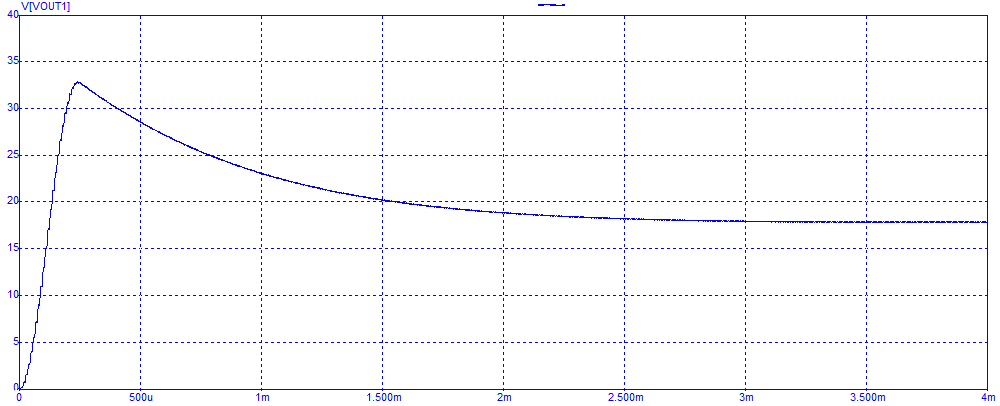
\includegraphics[width = 13.5cm]{Vout 19V.png}
  \caption{Spanning aan de uitgang}
\end{figure}

\begin{figure}[h!]
  \centering
  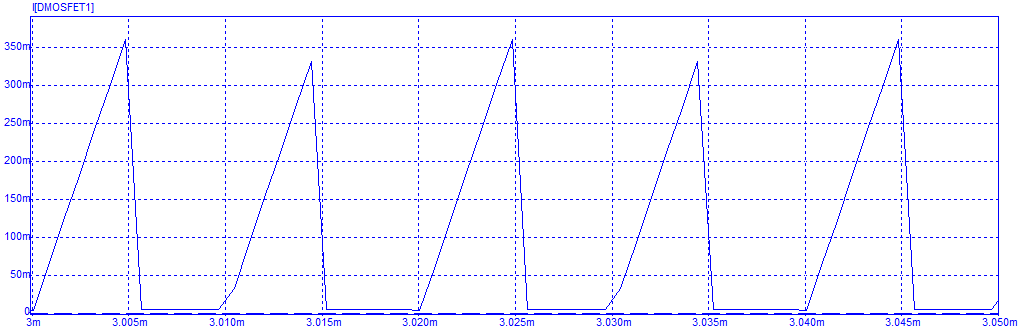
\includegraphics[width = 13.5cm]{Ids 19V.png}
  \caption{Stroom door de Mosfet}
\end{figure}

\begin{figure}[h!]
  \centering
  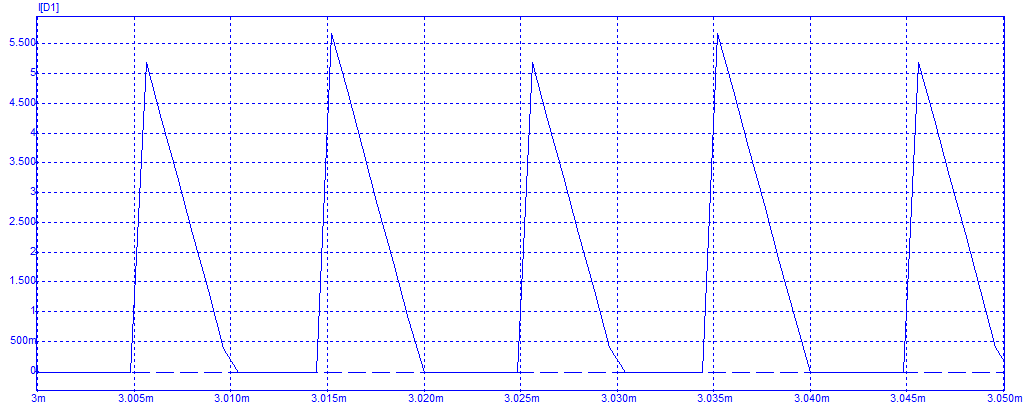
\includegraphics[width = 13.5cm]{Id 19V.png}
  \caption{Stroom door de diode}
\end{figure}


\subsection{Schakeling 19V}

\begin{figure}[h!]
  \centering
  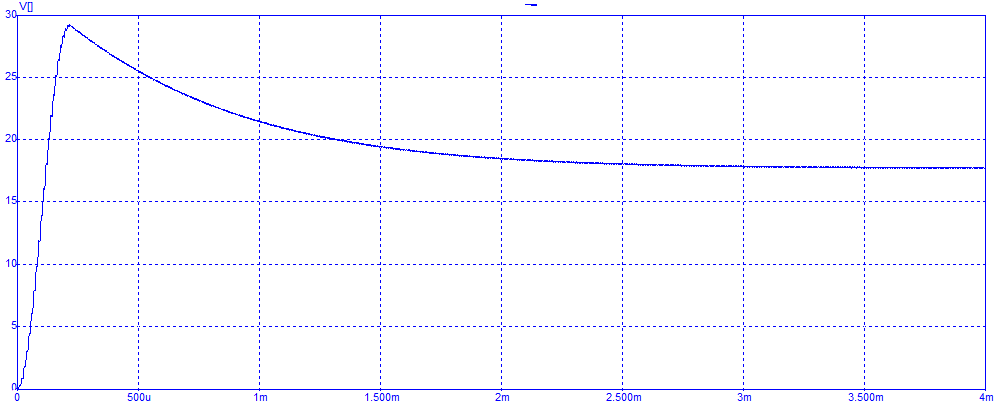
\includegraphics[width = 13.5cm]{Vout 15V.png}
  \caption{Spanning aan de uitgang}
\end{figure}

\begin{figure}[h!]
  \centering
  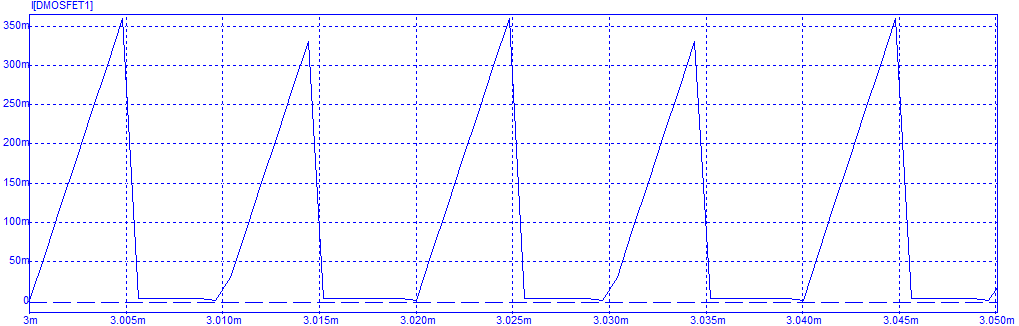
\includegraphics[width = 13.5cm]{Ids 15V.png}
  \caption{Stroom door de Mosfet}
\end{figure}

\begin{figure}[h!]
  \centering
  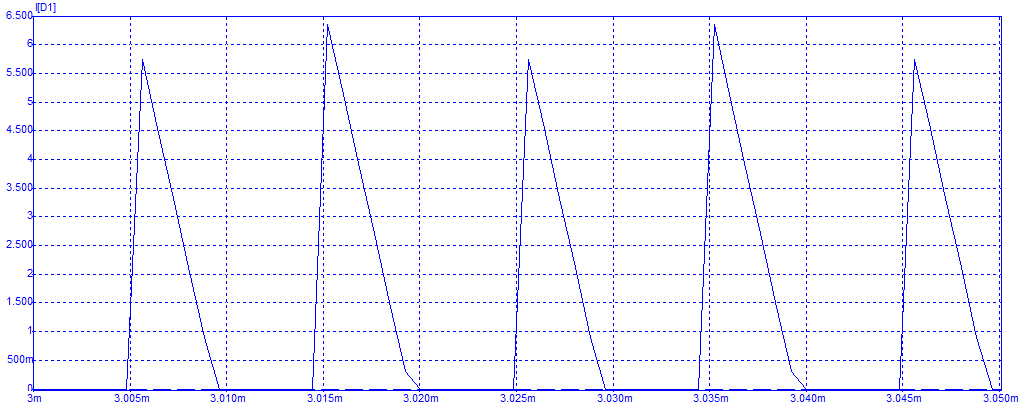
\includegraphics[width = 13.5cm]{Id 15V.png}
  \caption{Stroom door de diode}
\end{figure}


\subsection{Schakeling 19V}

\begin{figure}[h!]
  \centering
  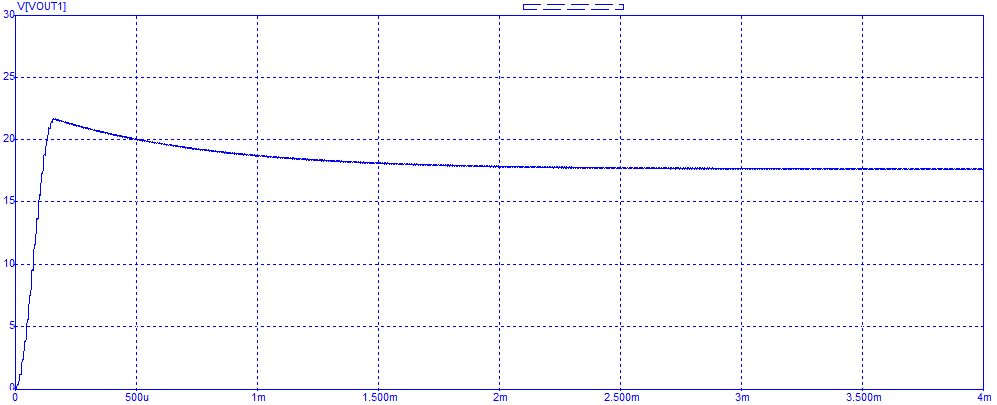
\includegraphics[width = 13.5cm]{Vout 12V.png}
  \caption{Spanning aan de uitgang}
\end{figure}

\begin{figure}[h!]
  \centering
  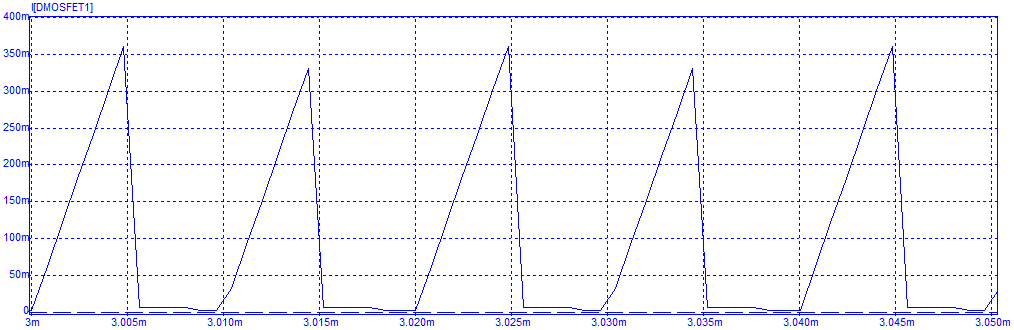
\includegraphics[width = 13.5cm]{Ids 12V.png}
  \caption{Stroom door de Mosfet}
\end{figure}

\begin{figure}[h!]
  \centering
  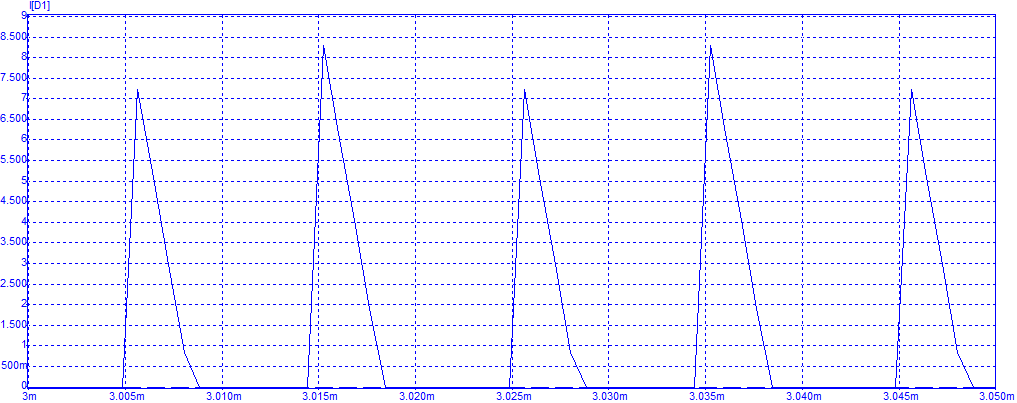
\includegraphics[width = 13.5cm]{Id 12V.png}
  \caption{Stroom door de diode}
\end{figure}




.

\end{document}
